%% TEMPLATE RELAZIONE TIROCINIO TEORIA DEI SISTEMI 
%% 
%% Decision & Control Lab
%% Politecnico di Bari
%% 
%% NON MODIFICARE i file presenti nella cartella 00-settings.
%%
%%%%%%%%%%%%%%%%%%%%%%%%%%%%%%%%%%%%%%%%%%%%%%%%%%%%%%%%%%%%%%%
% Impostazioni e installazione dei pacchetti (NON MODIFICARE) 
\documentclass{00-settings/document}
\usepackage{00-settings/style}   

%%%%%%%%%%%%%%%%%%%%%%%%%%%%%%%%%%%%%%%%%%%%%%%%%%%%%%%%%%%%%%%
% CONFIGURA QUI: tutte le informazioni della relazione si cambiano
% modificando solo questo blocco, non serve toccare altri file.
%%%%%%%%%%%%%%%%%%%%%%%%%%%%%%%%%%%%%%%%%%%%%%%%%%%%%%%%%%%%%%%

% --- Lingua ---
\usepackage[italian]{babel}       % Relazione in italiano
%\usepackage[english]{babel}      % Relazione in inglese: commentare la riga sopra e decommentare questa

% --- Informazioni personali ---
\newcommand{\studenti}{Nome Cognome (aggiungere firma)}
\newcommand{\tutor}{Nome Cognome (aggiungere firma)}
\newcommand{\corsodilaurea}{INGEGNERIA <......>}
\newcommand{\tipo}{interno}        % interno / esterno
\newcommand{\periododa}{24/04/2024}
\newcommand{\periodoa}{24/04/2025}

% --- Loghi del frontespizio ---
% Per cambiare un logo basta sostituire il percorso del file qui sotto.
% Metti la tua immagine (png/jpg/pdf) nella cartella 00-settings e indica il percorso.
\renewcommand{\logosinistra}{00-settings/poliba.png}  % logo in alto a sinistra
\renewcommand{\logodestra}{00-settings/dmmm.png}      % logo in alto a destra
%%
%%%%%%%%%%%%%%%%%%%%%%%%%%%%%%%%%%%%%%%%%%%%%%%%%%%%%%%%%%%%%%%
%%
%%
%%%%%%%%%%%%%%%%%%%%%%%%%%%%%%%%%%%%%%%%%%%%%%%%%%%%%%%%%%%%%%%
% FRONTESPIZIO (NON MODIFICARE) 
\begin{document}
\maketitle
%%%%%%%%%%%%%%%%%%%%%%%%%%%%%%%%%%%%%%%%%%%%%%%%%%%%%%%%%%%%%%%
%%
%%%%%%%%%%%%%%%%%%%%%%%%%%%%%%%%%%%%%%%%%%%%%%%%%%%%%%%%%%%%%%%
% INIZIO DEL DOCUMENTO
\section{OBIETTIVI}
In questa sezione si presenta brevemente il contesto in cui si è svolto il tirocinio e gli obiettivi concordati con il tutor accademico (e, se presente, con il tutor aziendale) prima dell'inizio dell'attività. Va indicato cosa ci si proponeva di imparare o realizzare, perché quell'attività era rilevante rispetto al proprio percorso di studi, e quali competenze si intendeva acquisire o consolidare. Non è necessario anticipare qui i risultati: questa sezione descrive le premesse, non l'esito.

\section{DESCRIZIONE DELL’AZIENDA/ENTE NEL QUALE È STATA SVOLTA L’ATTIVITÀ (solo per tirocini esterni)}
Per i tirocini esterni, questa sezione presenta l'azienda o l'ente ospitante: il settore in cui opera, le dimensioni, il tipo di attività svolta e, se rilevante, il gruppo o dipartimento specifico in cui si è stati inseriti. Lo scopo è dare al lettore il contesto organizzativo necessario per comprendere le attività descritte più avanti. Per i tirocini interni (svolti presso il Decision \& Control Lab) questa sezione va rimossa.

\section{ATTIVITÀ SVOLTE}
Questa è la sezione centrale della relazione: descrive in dettaglio cosa è stato fatto durante il tirocinio. È utile organizzarla in ordine cronologico o per macro-attività, spiegando per ciascuna: qual era il compito, quale approccio o metodologia è stata usata, quali strumenti software o tecniche sono stati impiegati, ed eventuali difficoltà incontrate e come sono state affrontate. Se il lavoro ha previsto lo sviluppo di codice, è il punto in cui descriverlo e, se utile, includerne degli estratti (vedi \S\ref{appendiceA:codice} in appendice per come inserirlo).

\section{RISULTATI CONSEGUITI}
In questa sezione si riportano gli esiti concreti del tirocinio: cosa è stato consegnato o realizzato, in che misura gli obiettivi definiti in apertura sono stati raggiunti, e una valutazione critica del proprio lavoro (cosa ha funzionato, cosa si sarebbe potuto fare diversamente). È il luogo adatto anche per riflettere brevemente su cosa si è imparato dal punto di vista tecnico e professionale, ed eventualmente su possibili sviluppi futuri dell'attività svolta.

%%%%%%%%%%%%%%%%%%%%%%%%%%%%%%%%%%%%%%%%%%%%%%%%%%%%%%%%%%%%%%%
%% FINE DEL DOCUMENTO
%%
%%
%%
%%%%%%%%%%%%%%%%%%%%%%%%%%%%%%%%%%%%%%%%%%%%%%%%%%%%%%%%%%%%%%%

\appendix
\section{Appendice: Guida all'uso di \LaTeX{} (da rimuovere)}
Vi consigliamo di leggere questa guida direttamente dalla visualizzazione in PDF. 

\subsection*{Impostazione della lingua}
Un primo passo utile su Overleaf è modificare la lingua del controllo ortografico. Per farlo:

\begin{enumerate}
    \item Cliccare su \textbf{Menu} in alto a sinistra.
    \item Scorrere fino alla sezione \textbf{Spell check}.
    \item Selezionare la lingua desiderata (es. Italiano).
\end{enumerate}

\subsection*{Struttura del documento}
Per definire le sezioni principali del documento si usa il comando:
\begin{verbatim}
\section{Titolo della sezione}
\end{verbatim}

Per le sottosezioni:
\begin{verbatim}
\subsection{Titolo della sottosezione}
\end{verbatim}

È possibile creare ulteriori livelli con comandi come \verb|\subsubsection|.

\textit{Per separare due paragrafi, è sufficiente lasciare una riga vuota. \LaTeX{} aggiungerà automaticamente l'indentazione.}

Per formattare il testo:
\begin{verbatim}
\textit{corsivo}, \textbf{grassetto}
\end{verbatim}

\subsection{Riferimenti bibliografici}
La gestione delle fonti in \LaTeX{} si basa su un file \texttt{.bib}, ad esempio \texttt{references.bib}. Per aggiungere nuove voci:

\begin{itemize}
    \item Cercare l'articolo su \url{https://scholar.google.com}
    \item Cliccare su \textit{"Cita"} > \textit{BibTeX} e copiare il codice
    \item Incollare il codice nel file \texttt{.bib}
\end{itemize}

Per citare nel testo:
\begin{verbatim}
\cite{nomeRiferimento}
\end{verbatim}

Guida utile: \url{https://texblog.org/2014/04/22/using-google-scholar-to-download-bibtex-citations/}

\subsection{Equazioni}
Le equazioni si scrivono così:
\begin{verbatim}
\begin{equation}
\label{eq:esempio}
a^2 + b^2 = c^2
\end{equation}
\end{verbatim}

Per riferirsi all'equazione nel testo:
\begin{verbatim}
\eqref{eq:esempio}
\end{verbatim}

Equazioni più lunghe:
\begin{verbatim}
\begin{multline}
\label{eq:lunga}
J_i = \sum_{h=1}^{H} K_h + \\
+ \sum_{h=1}^{H} W_i
\end{multline}
\end{verbatim}

Formule nel testo: \verb|$f = \sum_d k$|

\begin{equation}
\label{eq:equazioneEsempio}
\int_{i=1}^{N}10x_{20}=\gamma \frac{10}{b_{10}^{4}}, \quad \forall i
\end{equation}

\begin{multline}
J_i(x_{i},\boldsymbol {x}_{-i} ,\boldsymbol {\bar{\omega}})  =\sum_{h=1}^{H} K_{h} (\boldsymbol l_{-i}(h) + e_i(h) + \delta^{T} x_{i}(h)- \bar{\omega}(h)) \cdot \\
 \cdot (e_i(h) +\delta^{T} x_{i}(h))  + \sum_{h=1}^{H} W_{i} (\delta_{g}^{T} x_{i}(h))
\label{eq:equazioneEsempioLunga}
\end{multline}

\subsection{Algoritmi}
\begin{verbatim}
\begin{algorithm}[h]
\caption{Nome dell'algoritmo}
\begin{algorithmic}
\STATE $\lambda^{+} = \mathrm{proj}_{\mathbb{R}^m_{\geq 0}}\left[\lambda$
\FOR{$i = 1, ..., N$}
    \IF{$i \in \mathcal{N_D}$}
        \STATE Calcola $\boldsymbol{\bar{\omega}}$
    \ELSIF{$i \in \mathcal{N_S}$}
        \STATE Imposta $\hat{J}_i^M$
    \ENDIF
\ENDFOR
\end{algorithmic}
\end{algorithm}
\end{verbatim}

\subsection{Teoremi, definizioni, ecc.}
Sono disponibili anche gli ambienti "teorema", "definizione", "lemma" e "corollario", numerati automaticamente:
\begin{verbatim}
\begin{teorema}
Enunciato del teorema.
\end{teorema}
\end{verbatim}
\begin{teorema}
Enunciato del teorema.
\end{teorema}

\subsection{Elenchi}
Elenchi puntati:
\begin{verbatim}
\begin{itemize}
\item Primo punto
\item Secondo punto
\end{itemize}
\end{verbatim}

Elenchi numerati:
\begin{verbatim}
\begin{enumerate}
\item Primo punto
\item Secondo punto
\end{enumerate}
\end{verbatim}

Multilivello:
\begin{verbatim}
\begin{itemize}
\item Primo livello
    \begin{enumerate}
    \item Secondo livello
    \end{enumerate}
\end{itemize}
\end{verbatim}

\subsection{Tabelle}
\begin{verbatim}
\begin{table}[h]
\centering
\caption{Titolo tabella}
\label{tab:esempio}
\begin{tabular}{cccc}
 & Top & Bottom & Left/Right \\
\hline
Prima & 3.5 & 2.5 & 1.5 \\
Restante & 2.5 & 2.5 & 1.5 \\
\end{tabular}
\end{table}
\end{verbatim}

Tool utile per generare tabelle da Excel: \cite{CreateLaTexTable}

\subsection{Immagini}
Per inserire un'immagine:

\begin{verbatim}
\begin{figure}[t!]
\centering
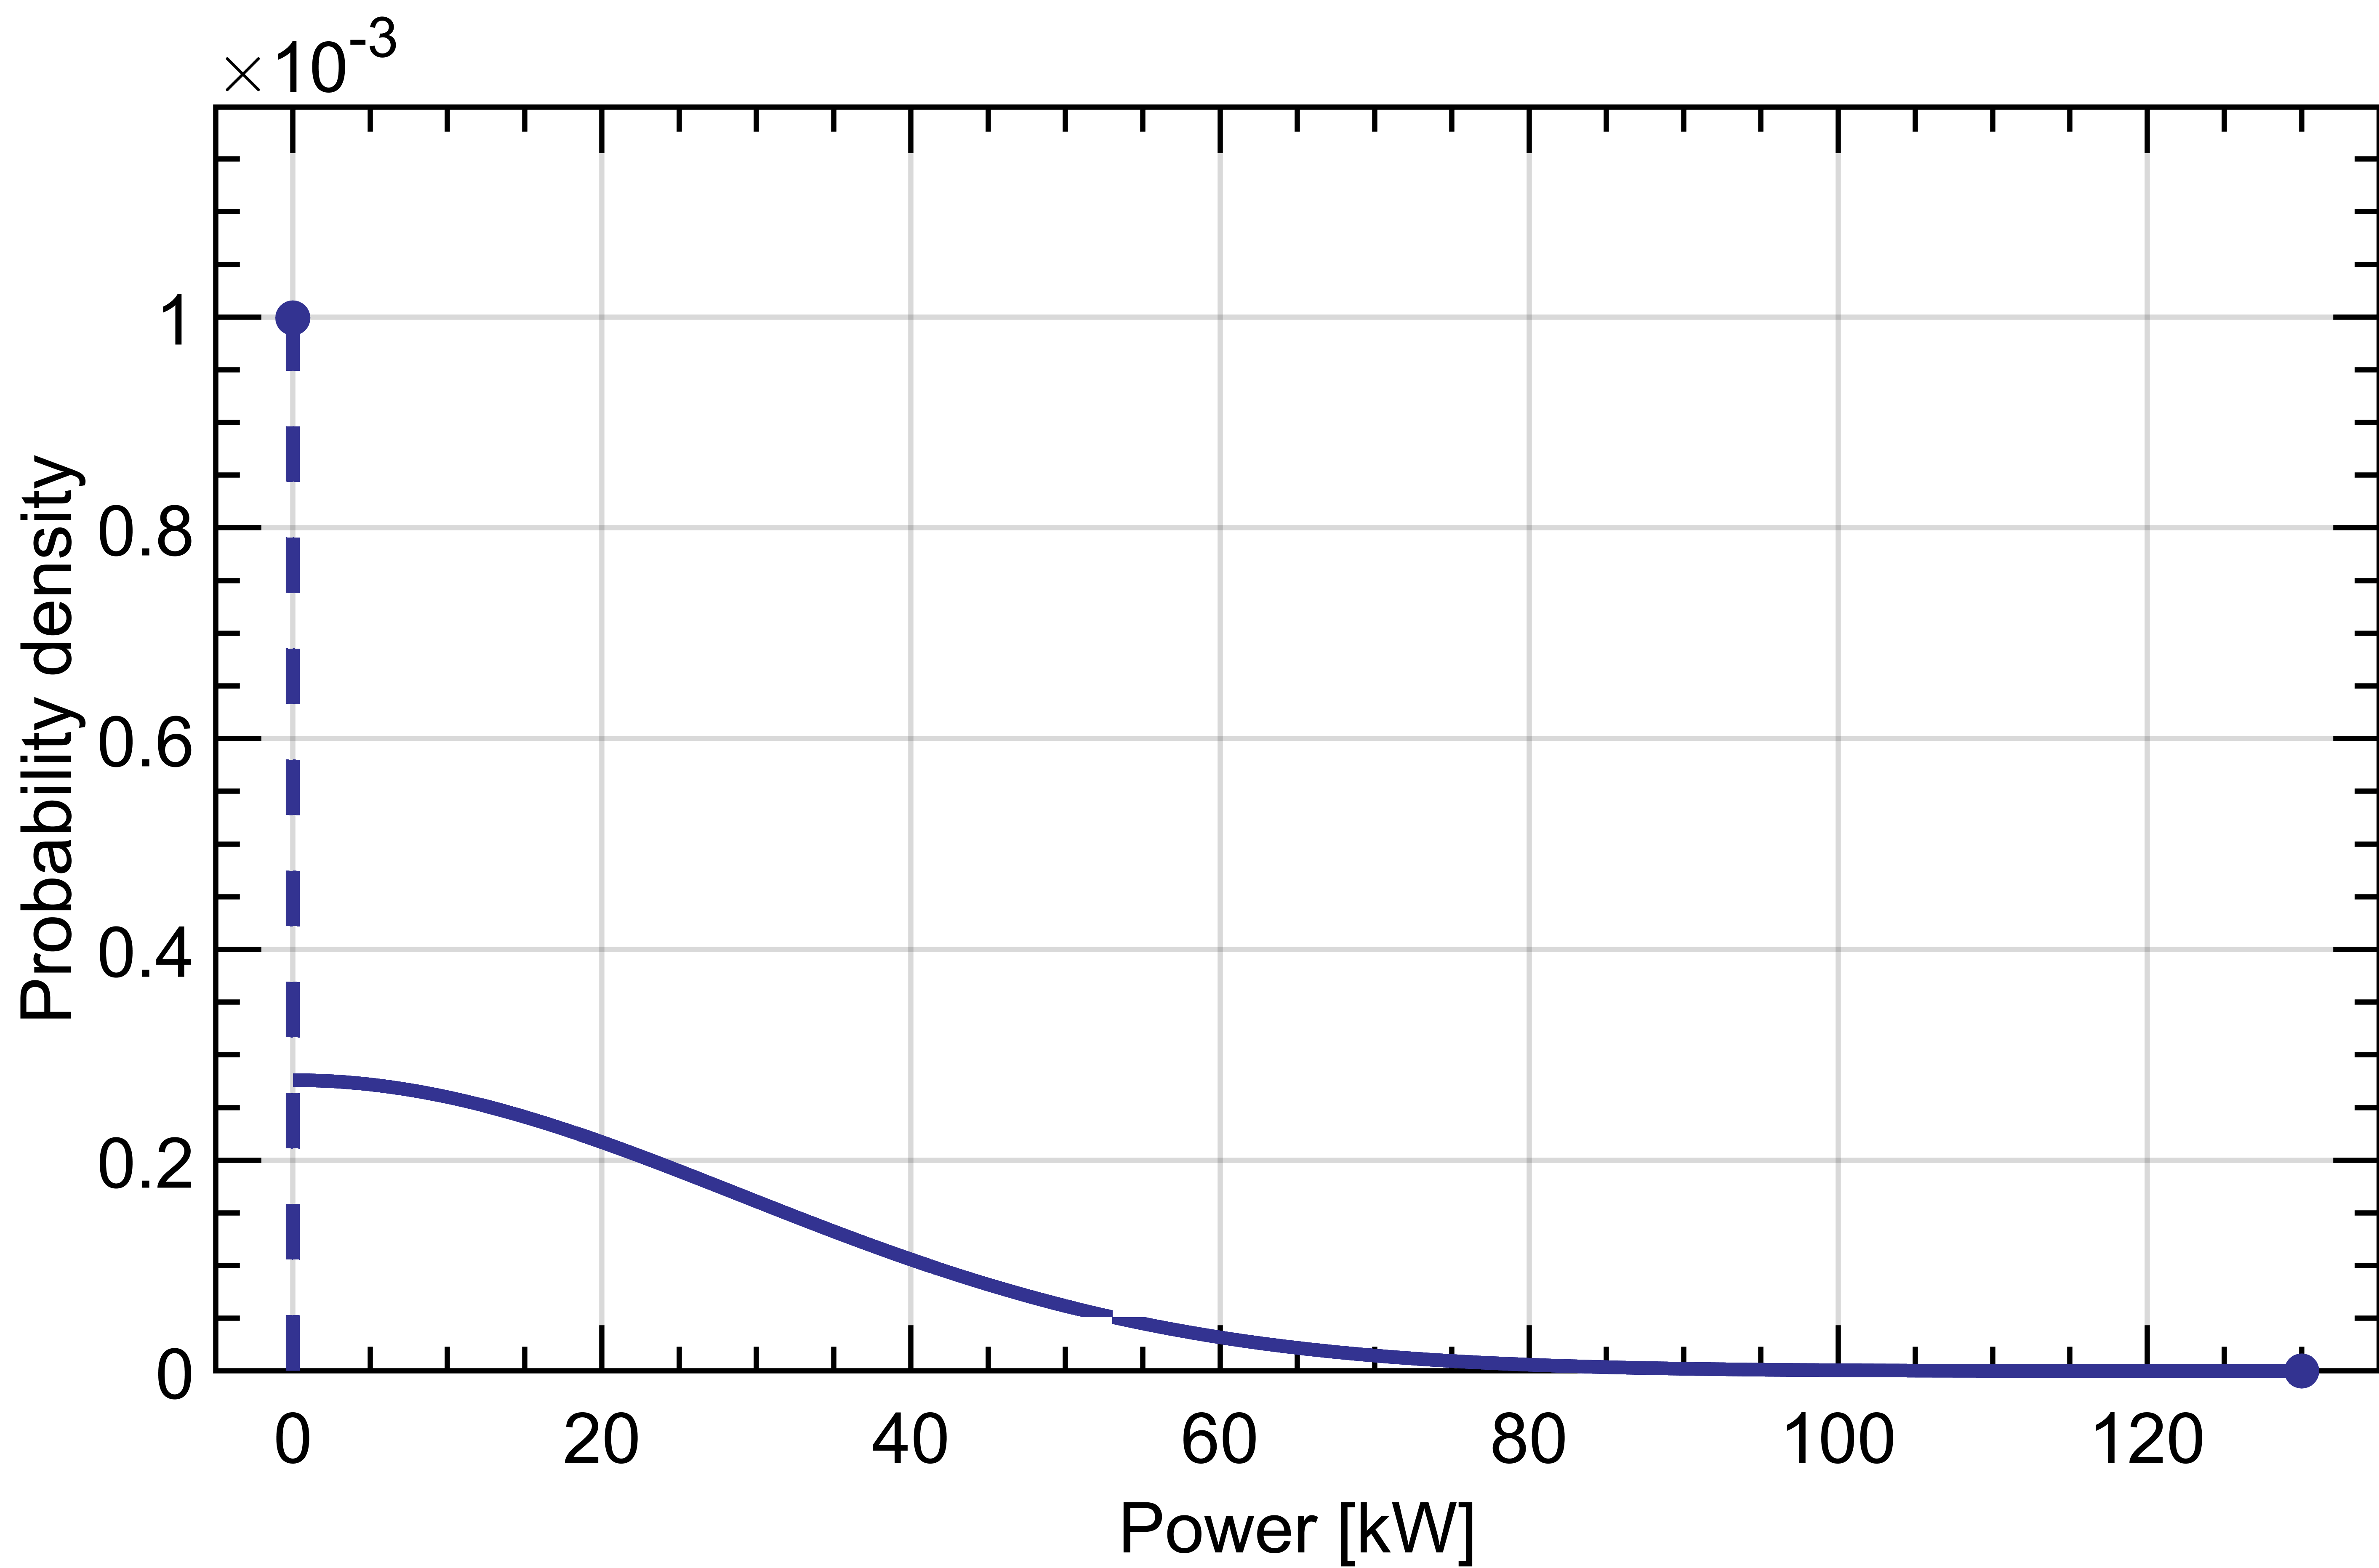
\includegraphics[width=0.5\textwidth]{02-figures/esempioFigura.png}
\caption{Esempio figura.}
\label{fig:Prova}
\end{figure}
\end{verbatim}

Suggerimenti:

\begin{itemize}
\item Usare \verb|~| in \verb|Fig.~\ref{fig:Prova}| per evitare la separazione su due righe
\item Usare immagini in `.pdf` o `.eps` per una qualità migliore
\item Usare opzioni di posizionamento come `[h]`, `[t]`, `[b]`, `[H]`, `[!ht]`
\end{itemize}

\begin{verbatim}
\begin{figure}[h]
\centering
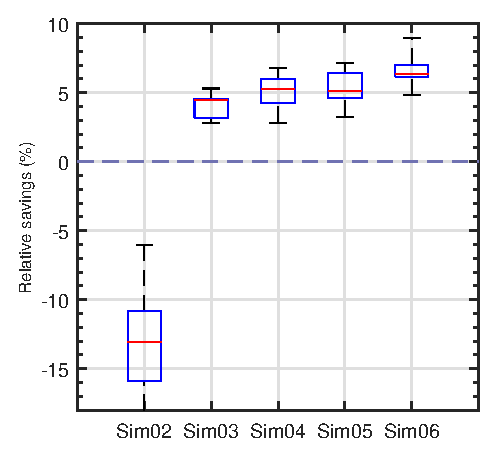
\includegraphics[width=0.5\textwidth]{02-figures/esempioFigura2.eps}
\caption{Esempio figura in formato eps.}
\label{fig:Prova2}
\end{figure}

\begin{figure}[H]
\centering
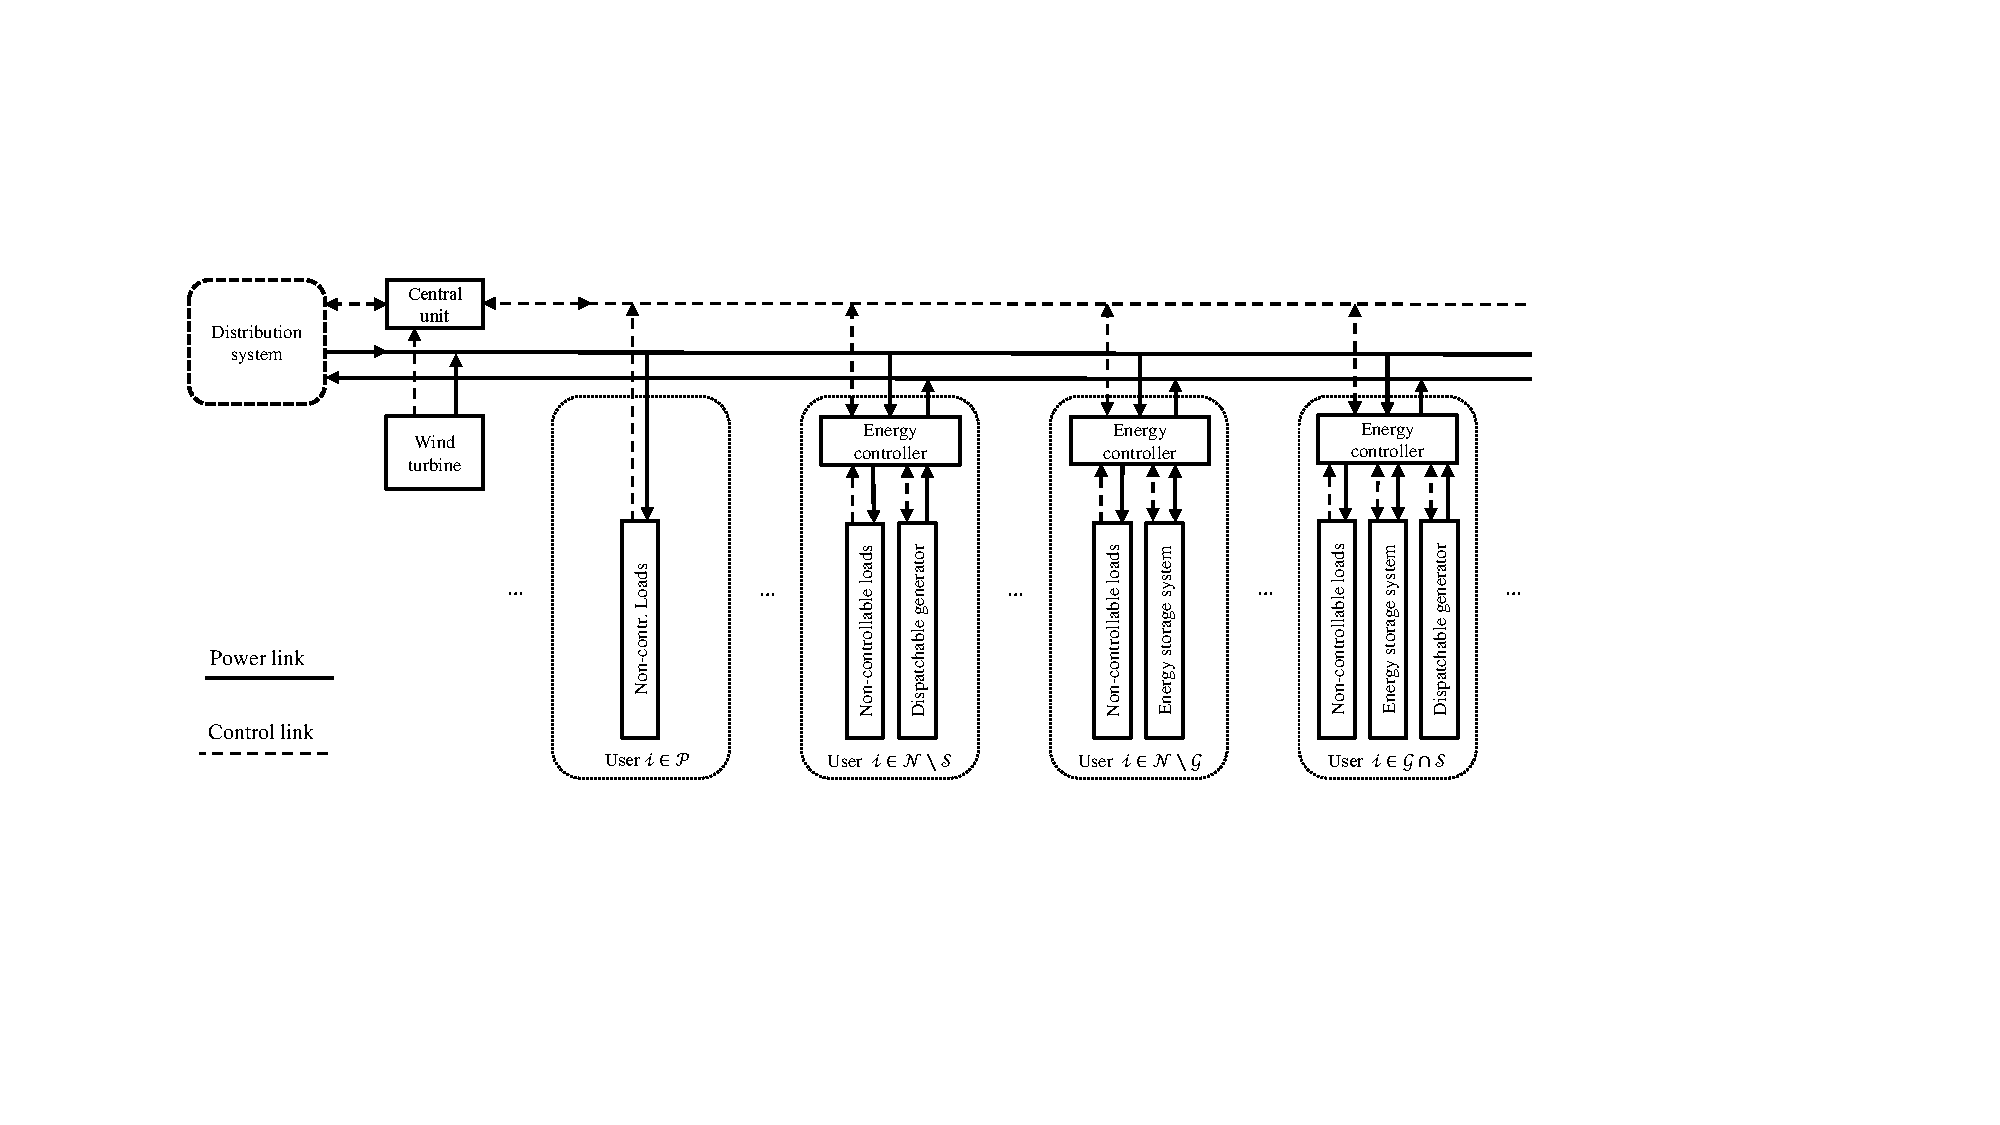
\includegraphics[width=0.8\textwidth]{02-figures/esempioFigura3.pdf}
\caption{Esempio figura in pdf.}
\label{fig:Prova3}
\end{figure}
\end{verbatim}

Ulteriori dettagli: \url{https://it.overleaf.com/learn/latex/Positioning_of_Figures}

\subsection{Codice sorgente}
\label{appendiceA:codice}
Se durante il tirocinio avete scritto del codice (Matlab, Python, ecc.) potete includerlo direttamente nella relazione. Mettete il file nella sottocartella del linguaggio (03-code/matlab oppure 03-code/python) e richiamatelo con "lstinputlisting":

\begin{verbatim}
\lstinputlisting{03-code/matlab/nomefile.m}
\lstinputlisting[style=pythonstyle]{03-code/python/nomefile.py}
\end{verbatim}

Esempio (Matlab):
\lstinputlisting{03-code/matlab/Codice1.m}

Esempio (Python, con lo stile "pythonstyle" già definito nel pacchetto del laboratorio):
\lstinputlisting[style=pythonstyle]{03-code/python/Codice1.py}




%%%%%%%%%%%%%%%%%%%%%%%%%%%%%%%%%%%%%%%%%%%%%%%%%%%%%%%%%%%%%%%
% STAMPA DELLA BIBLIOGRAFIA (NON MODIFICARE
\printbibliography[heading=bibintoc,title={Riferimenti}]
%\printbibliography[heading=bibintoc,title={References}] % Per tesina in inglese decommentare
%%%%%%%%%%%%%%%%%%%%%%%%%%%%%%%%%%%%%%%%%%%%%%%%%%%%%%%%%%%%%%%
\end{document}
% FINE